\section{Результаты численного моделирования}

В настоящем разделе описаны результаты двух видов расчетов. Во-первых, проведенной верификации модели экипажа на плоскости с регуляризованным сухим трением в сравнении с безынерционной моделью. Сравнение устроено при стремлении доли массы ролика в общей массе омни-колеса к нулю. Во-вторых, качественно сравнивается движение экипажа на плоскости с вязким трением с достаточно большим коэффициентом и движение модели, построенной в главах 1 и 2.

\subsection{Верификация модели с сухим трением}

Для проверки взаимной корректности безынерционной модели и модели с сухим трением проведены численные испытания, в которых, при прочих равных, изменялась величина $\massrel$ -- отношение массы одного ролика к массе колеса в целом. В этом случае оказалось, что при уменьшении данного параметра движение экипажа и омни-колес неограниченно приближаются к соответствующим функциям решения задачи Коши, получаемым в силу дифференциальных уравнений движения, используемых в работе~\cite{Borisov2011}, в которых динамика роликов не учитывается. При этом остальные параметры экипажа, такие как массы его частей, их моменты инерции, геометрические размеры, положения, а также начальные данные -- скорость центра масс и угловая скорость платформы, задавались согласованными между двумя моделями. Как и в главах 1 и 2, рассматривается симметричная конфигурация экипажа. Однако концы роликов в данном рассмотрении не усекаются: в силу выбора модели контактных сил и построенного явного алгоритма отслеживания контакта, особенность на острии ролика не препятствует проведению расчетов. Количество роликов $n$ равно $4$. Рассмотрены два типа начальных условий $\vec{v}(0) = (v_0, 0, 0)^T, \omega(0) = \omega_0$ (см. рис.~\ref{fig:my_exp_setup}):
\begin{enumerate}
\item экипаж имеет начальную линейную скорость в направлении одного из колес и не закручен (ожидаемый результат - центр масс экипажа движется вдоль оси $Ox$, экипаж не вращается),
\item экипаж закручен вокруг вертикальной оси, проходящей через его центр масс, скорость центра масс равна нулю (ожидаемый результат - экипаж вращается вокруг своей вертикальной оси симметрии, и центр масс покоится).
\end{enumerate}
Значения отношения $\massrel$ массы ролика к общей массе колеса принимали в обоих случаях значения от $10^{-6}$ до $10^{-1}$ с шагом $1$ по порядку малости.

\begin{figure}[!ht]
    \centering
    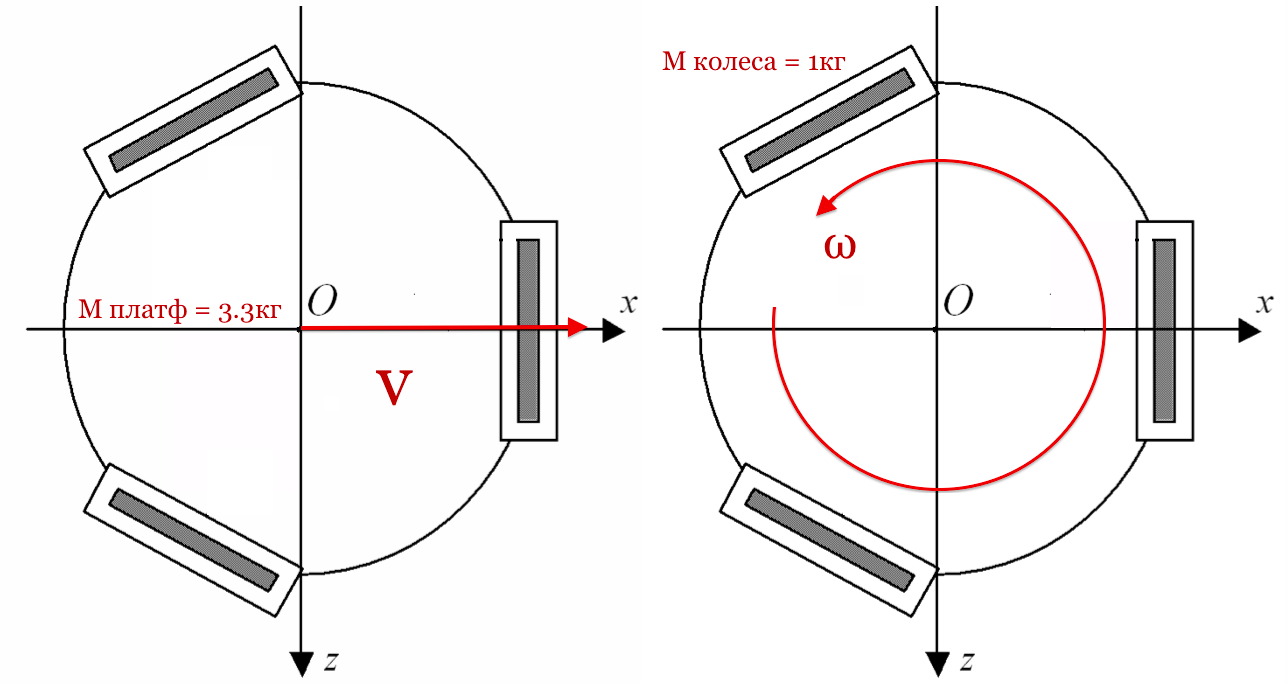
\includegraphics[width=0.95\textwidth]{content/parts/3_friction/diploma/img/art/my_exp_setup.png}
    \caption{Параметры экспериментов}
    \label{fig:my_exp_setup}
\end{figure}

В таблице\upr{tab:verif} приведены величины отличий угла курса $\theta$ экипажа и координат центра масс $x, y$ к моменту безразмерного времени $t = 10$. Отличия уменьшаются с уменьшением порядка величины отношения массы одного ролика $m_{\text{рол}}$ к суммарной массе колеса $m_{\text{к}}$.

\begin{table}[]\label{tab:verif}
    \begin{tabular}{l|l|l}
     & Движение $1$ & Движение $2$ \\ \hline
    $\frac{m_{\text{рол}}}{m_{\text{к}}}$ &
    $\Delta \theta$ &
    $\max(|\Delta x|, |\Delta y|)$ \\ \hline
    $10^{-1}$ & $\approx 1$       & $\approx 1$       \\
    $10^{-2}$ & $\approx 10^{-1}$ & $\approx 0.5$     \\
    $10^{-3}$ & $\approx 10^{-2}$ & $\approx 10^{-1}$ \\
    $10^{-4}$ & $\approx 10^{-3}$ & $\approx 10^{-2}$ \\
    $10^{-5}$ & $\approx 10^{-3}$ &                   \\
    $10^{-6}$ & $\approx 10^{-4}$ & 
    \end{tabular}
    \caption{Порядок различий в значениях угла курса платформы $\theta$ и координат центра масс $x, y$ экипажа при движениях $1$ и $2$ и уменьшении $\massrel$}
\end{table}

На рис.~\ref{fig:exp_examples} приведены примеры траектории центра масс $y(x)$ и зависимости $\psi(t)$ угла поворота $\psi$ платформы вокруг вертикальной оси, проходящей через её центр, для случаев 1) и 2). Кривые $y(x)$, изображающие траектории центра масс, соответствуют, в сущности, точке -- началу координат -- в случае $v_0 = 0, \omega_0 = 1$, и отрезку прямой, совпадающей с осью $x$, в случае $v_0 = 1, \omega_0 = 0$, т.к. масштаб отображения таков, чтобы были видны отклонения от точных значений, возникающие в силу вычислительной погрешности, но сами эти отклонения имеют порядок малости, позволяющий считать их нулевыми. Аналогичное утверждение верно и для зависимости угла поворота платформы $\psi$ от времени в случае поступательного движения - полученная зависимость близка к постоянной.

Ниже представлены результаты нескольких численных экспериментов. Во всех случаях величины, изображенные на рис.~\ref{fig:exp_examples}, демонстрируют поведение, не различимое в масштабе рис.~\ref{fig:exp_examples}, и поэтому приведены лишь расхождения между построенной нами моделью и верификационной идеализацией, которые и представляют интерес. Также представлена абсолютная величина скорости скольжения в точке контакта в физической модели.

Графики зависимости скорости скольжения от времени показывают, что скольжение имеет место в окрестности момента смены роликов. Для вращательного движения это объясняется наличием того же динамического эффекта раскручивания роликов, что был обнаружен в главах 1 и 2: скользят именно вновь входящие в контакт ролики, но не ролики, уже находящиеся в контакте достаточное время. В случае поступательного движения платформы экипажа дополнительно возникает раскручивание роликов задних колес, находящихся в контакте, поскольку для идеального качения при подходе к острию, ролику необходима бесконечная угловая скорость собственного вращения, т.к. его радиус вблизи острия стремится к нулю.

Видно, что с ростом доли массы роликов в общей массе колеса скольжение в контакте становится существеннее, изменяясь от пренебрежимо малого при $\massrel = 10^{-6}$ до весьма существенного уже при $\massrel = 10^{-3}$. Тем не менее, расхождения траектории и угла поворота платформы малы, а скольжение наблюдается лишь в точках колеса, которые в промышленных конструкциях не присутствуют (см. Обзор), что и позволяет считать верификацию проведенной.
\newpage

% EXAMPLES
\begin{figure}[h]
\centering
\begin{subfigure}{.47\textwidth}
    \centering
    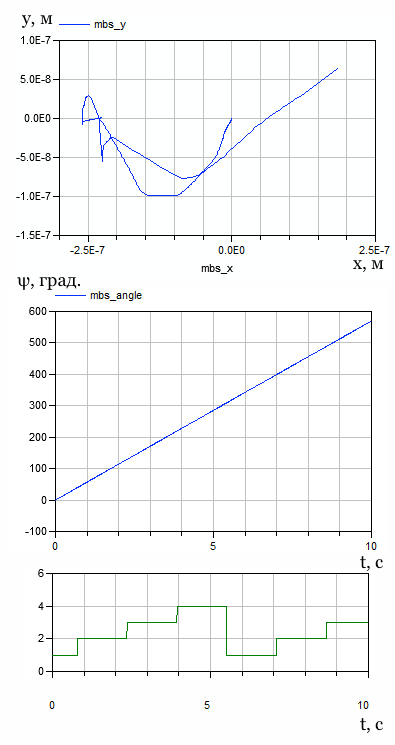
\includegraphics[width=\textwidth]{content/parts/3_friction/diploma/img/res/example_v_0_0_omega_1_frac_1e-1_n_4_time_10s.png}
    \caption{$\massrel = 0,1, v_0 = 0, \omega_0 = 1$}
    \label{fig:exp_example_omega}
\end{subfigure}%
\hspace{5pt}
\begin{subfigure}{.47\textwidth}
    \centering
    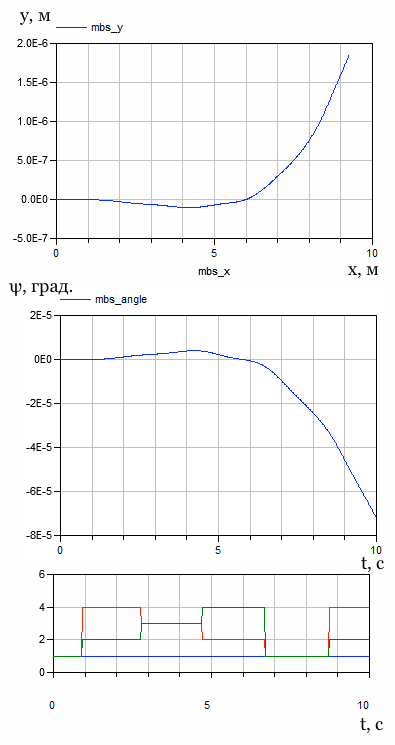
\includegraphics[width=\textwidth]{content/parts/3_friction/diploma/img/res/example_v_1_0_omega_0_frac_1e-1_n_4_time_10s.png}
    \caption{$\massrel = 0,1, v_0 = 1, \omega_0 = 0$}
    \label{fig:exp_example_v}
\end{subfigure}
\caption{Примеры траекторий, характера изменения угла и смены номеров роликов в контакте для двух типов начальных условий. На нижнем графике - номер ролика в контакте, см. рис.~\ref{OmniWheel}}
\label{fig:exp_examples}
\end{figure}
\newpage

\begin{figure}[h]
\begin{center}\begin{equation*}\begin{array}{cc}
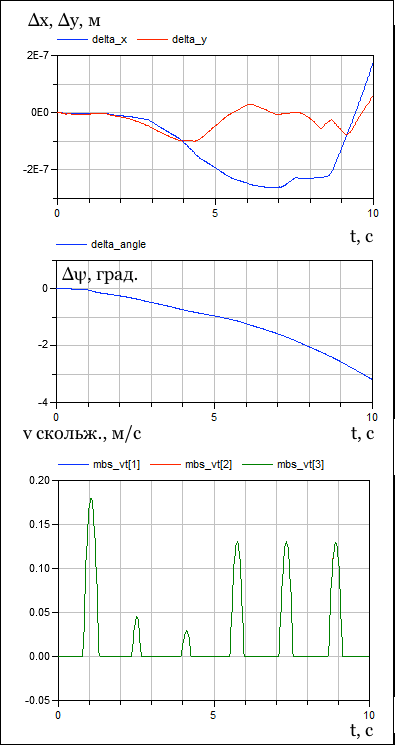
\includegraphics[width=7cm, viewport=0 0 395 745,clip]{content/parts/3_friction/diploma/img/res/comparison_v_0_0_omega_1_frac_1e-1_n_4_time_10s.png} & 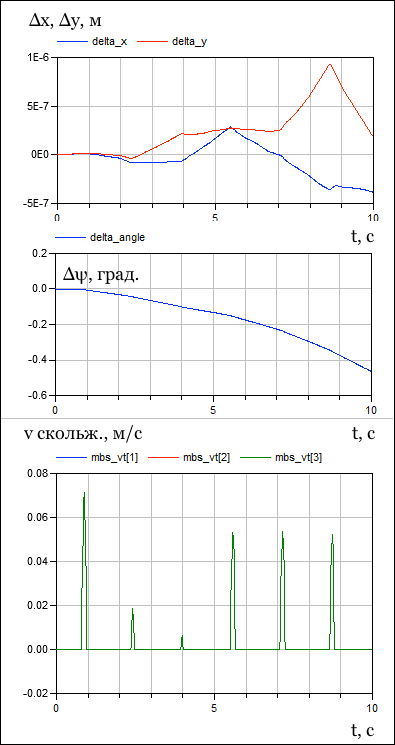
\includegraphics[width=7cm, viewport=0 0 395 745,clip]{content/parts/3_friction/diploma/img/res/comparison_v_0_0_omega_1_frac_1e-2_n_4_time_10s.png}\\
\massrel = 10^{-1}, v_0 = 0, \omega_0 = 1 & \massrel = 10^{-2}, v_0 = 0, \omega_0 = 1\\
\end{array}\end{equation*}\end{center}
\caption{Движение 1 экипажа на плоскости с сухим трением, $\massrel = 10^{-1}, 10^{-2}$}
\end{figure}
\newpage

\begin{figure}[h]
\begin{center}\begin{equation*}\begin{array}{cc}
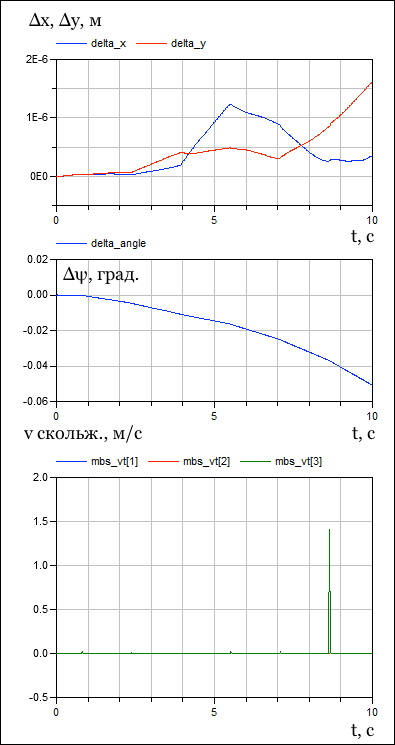
\includegraphics[width=7cm, viewport=0 0 395 745,clip]{content/parts/3_friction/diploma/img/res/comparison_v_0_0_omega_1_frac_1e-3_n_4_time_10s.png} & 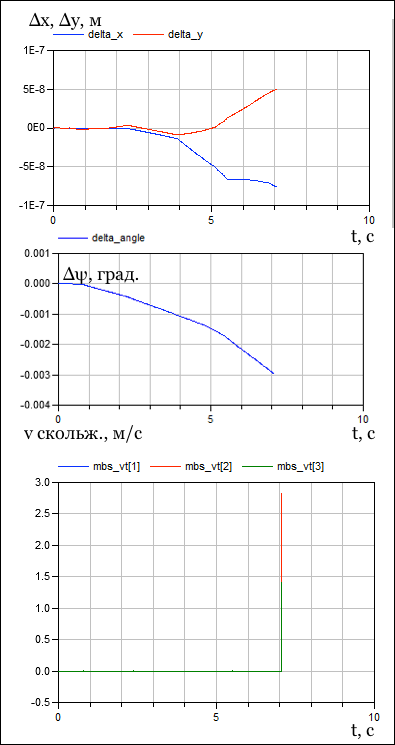
\includegraphics[width=7cm, viewport=0 0 395 745,clip]{content/parts/3_friction/diploma/img/res/comparison_v_0_0_omega_1_frac_1e-4_n_4_time_10s.png}\\
\massrel = 10^{-3}, v_0 = 0, \omega_0 = 1 & \massrel = 10^{-4}, v_0 = 0, \omega_0 = 1\\
\end{array}\end{equation*}\end{center}
\caption{Движение 1 экипажа на плоскости с сухим трением, $\massrel = 10^{-3}, 10^{-4}$}
\end{figure}
\newpage

\begin{figure}[h]
\begin{center}\begin{equation*}\begin{array}{cc}
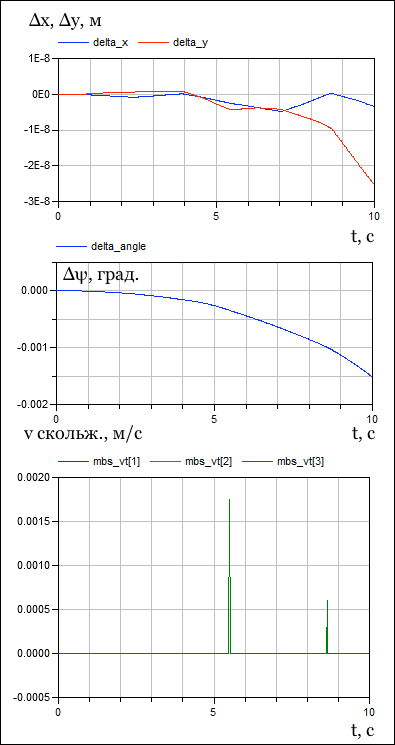
\includegraphics[width=7cm, viewport=0 0 395 745,clip]{content/parts/3_friction/diploma/img/res/comparison_v_0_0_omega_1_frac_1e-5_n_4_time_10s.png} & 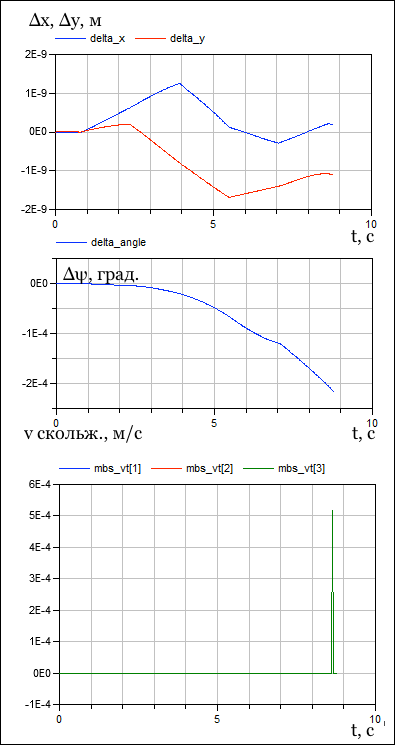
\includegraphics[width=7cm, viewport=0 0 395 745,clip]{content/parts/3_friction/diploma/img/res/comparison_v_0_0_omega_1_frac_1e-6_n_4_time_10s.png}\\
\massrel = 10^{-5}, v_0 = 0, \omega_0 = 1 & \massrel = 10^{-6}, v_0 = 0, \omega_0 = 1\\
\end{array}\end{equation*}\end{center}
\caption{Движение 1 экипажа на плоскости с сухим трением, $\massrel = 10^{-5}, 10^{-6}$}
\end{figure}
\newpage

\begin{figure}[h]
\begin{center}\begin{equation*}\begin{array}{cc}
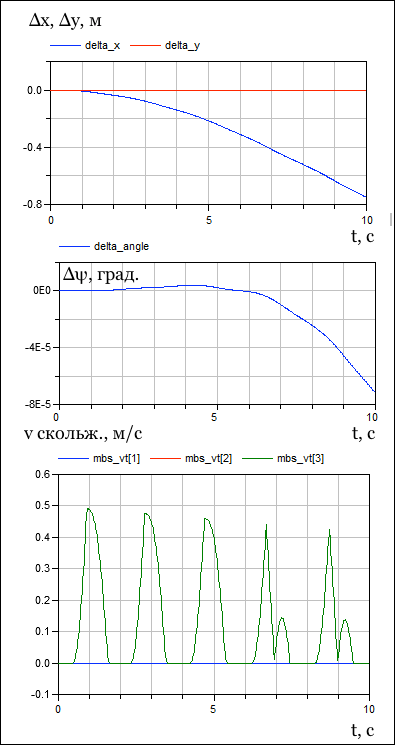
\includegraphics[width=7cm, viewport=0 0 395 745,clip]{content/parts/3_friction/diploma/img/res/comparison_v_1_0_omega_0_frac_1e-1_n_4_time_10s.png} & 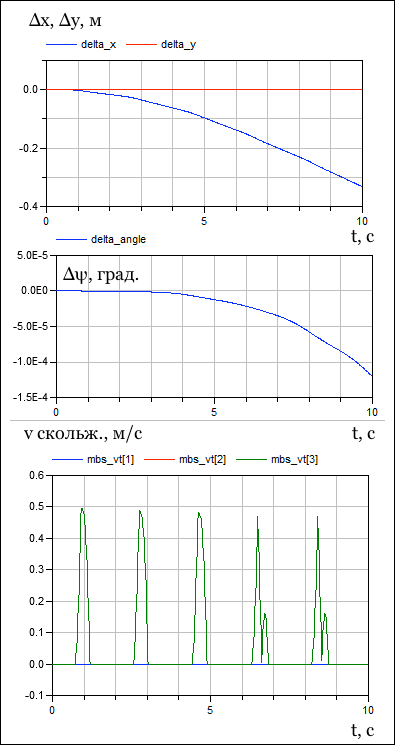
\includegraphics[width=7cm, viewport=0 0 395 745,clip]{content/parts/3_friction/diploma/img/res/comparison_v_1_0_omega_0_frac_1e-2_n_4_time_10s.png}\\
\massrel = 10^{-1}, v_0 = 1, \omega_0 = 0 & \massrel = 10^{-2}, v_0 = 1, \omega_0 = 0\\
\end{array}\end{equation*}\end{center}
\caption{Движение 2 экипажа на плоскости с сухим трением, $\massrel = 10^{-1}, 10^{-2}$}
\end{figure}
\newpage

\begin{figure}[h]
\begin{center}\begin{equation*}\begin{array}{cc}
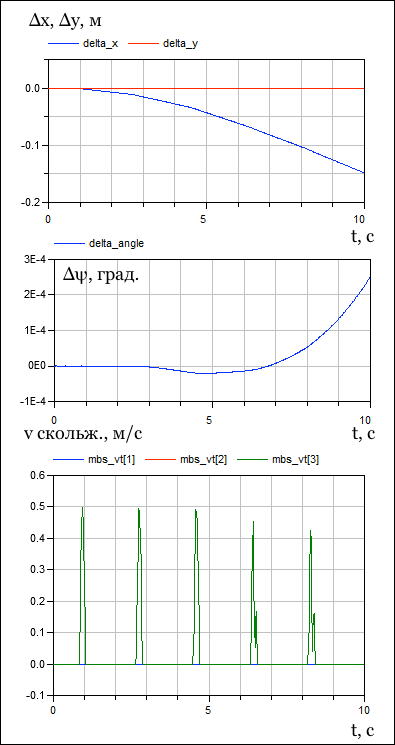
\includegraphics[width=7cm, viewport=0 0 395 745,clip]{content/parts/3_friction/diploma/img/res/comparison_v_1_0_omega_0_frac_1e-3_n_4_time_10s.png} & 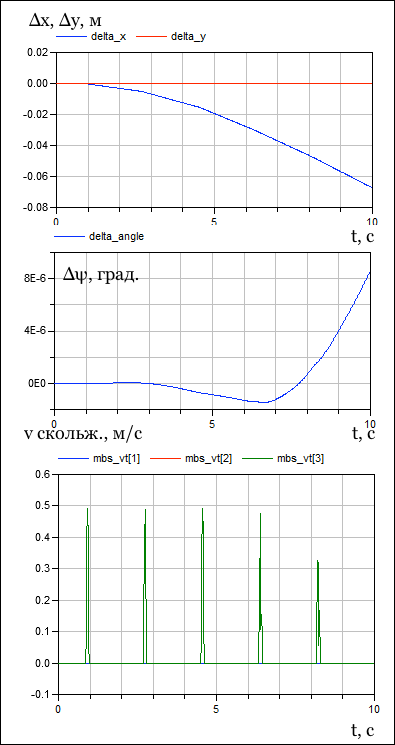
\includegraphics[width=7cm, viewport=0 0 395 745,clip]{content/parts/3_friction/diploma/img/res/comparison_v_1_0_omega_0_frac_1e-4_n_4_time_10s.png}\\
\massrel = 10^{-3}, v_0 = 1, \omega_0 = 0 & \massrel = 10^{-4}, v_0 = 1, \omega_0 = 0\\
\end{array}\end{equation*}\end{center}
\caption{Движение 1 экипажа на плоскости с сухим трением, $\massrel = 10^{-3}, 10^{-4}$}
\end{figure}
\newpage

% В процессе отладки модели рассматривались автономные движения отдельного омни-колеса.

Эволюция процесса контактирования для отдельного катящегося омни-колеса показана на Рис.~\ref{fig1}, где представлены зависимости расстояний $h$ между горизонтальной плоскостью и роликами одного и того же колеса, находящимися в разных фазах (перед контактом, в контакте, после контакта). Номер кривой соответствует номеру ролика на колесе. В увеличенном масштабе показан момент безударного гладкого переключения поверхностей контактирования роликов и горизонтальной плоскости.

\begin{figure}[htb]
\centerline{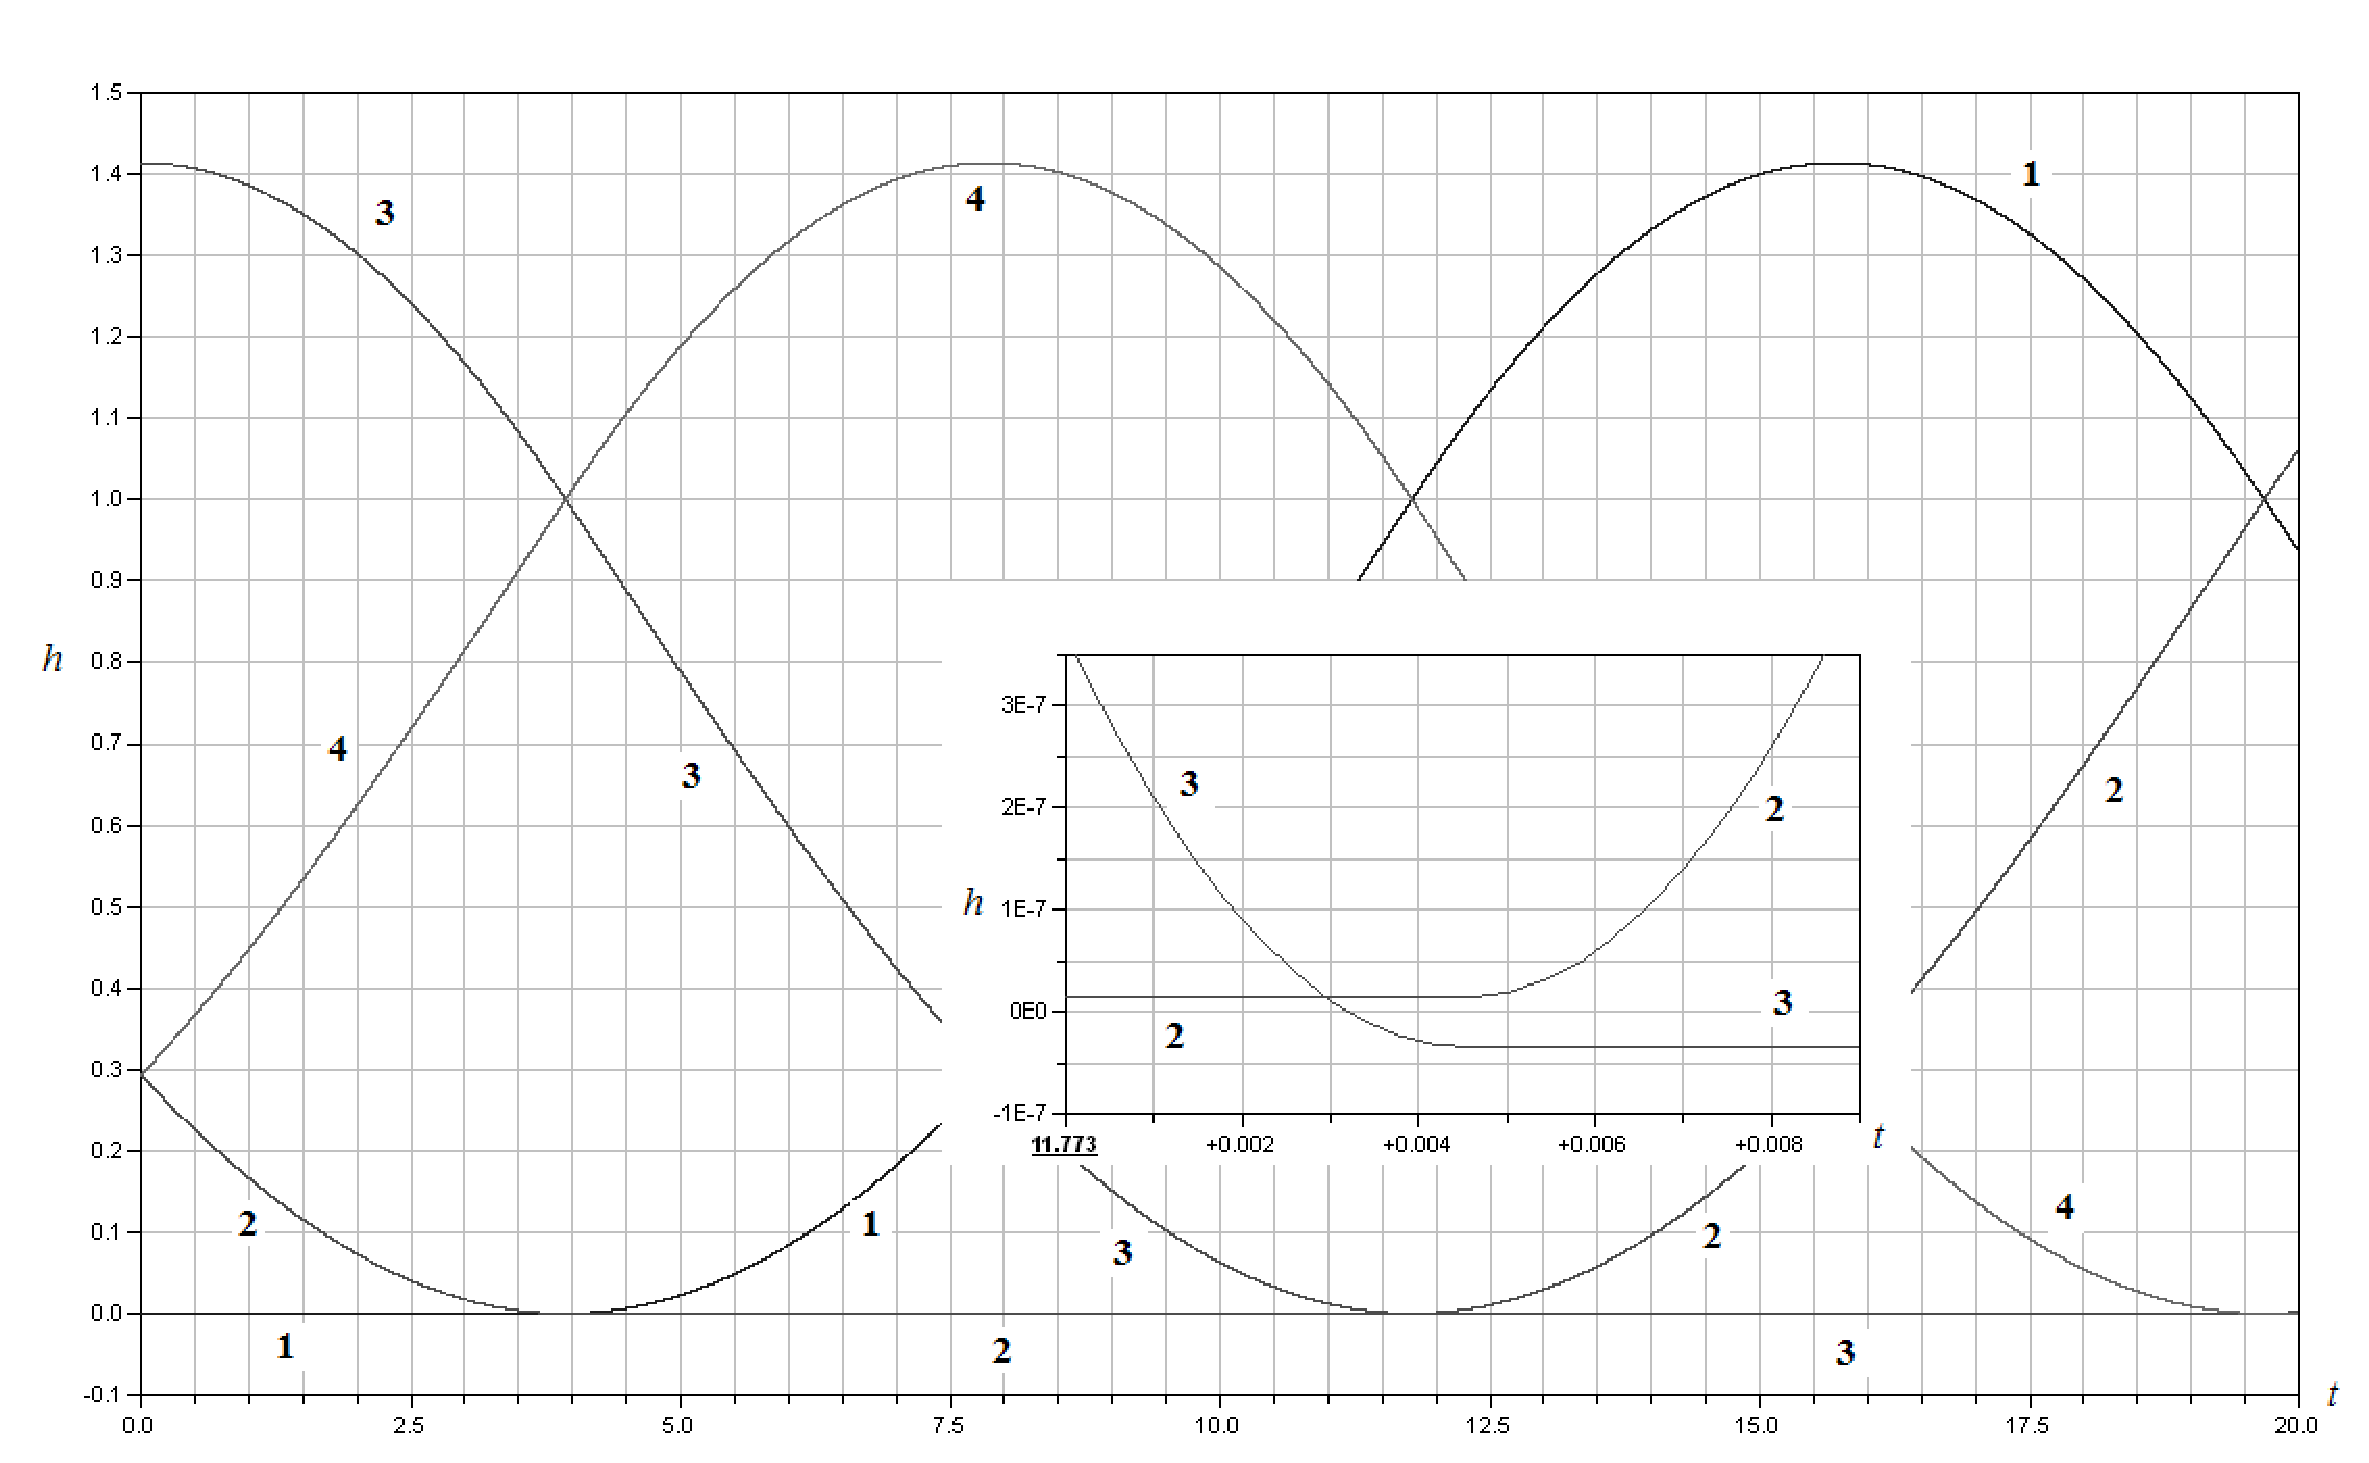
\includegraphics[width=15cm]{content/parts/3_friction/nd/Figure11.eps}}
\caption{Процесс смены роликов в контакте в численной модели.}
\label{fig1}
\end{figure}

Одновременно можно наблюдать точность соблюдения неудерживающей связи (Рис.~\ref{fig2}). Здесь обнаруживается процесс постепенного увеличения вычислительной ошибки -- расстояние между контактирующими телами медленно, для каждого последующего ролика в контакте, увеличивается. В то же время, абсолютная величина ошибки остается пренебрежимо малой -- около $10^{-7}$ от единицы длины. 

\begin{figure}[htb]
\centerline{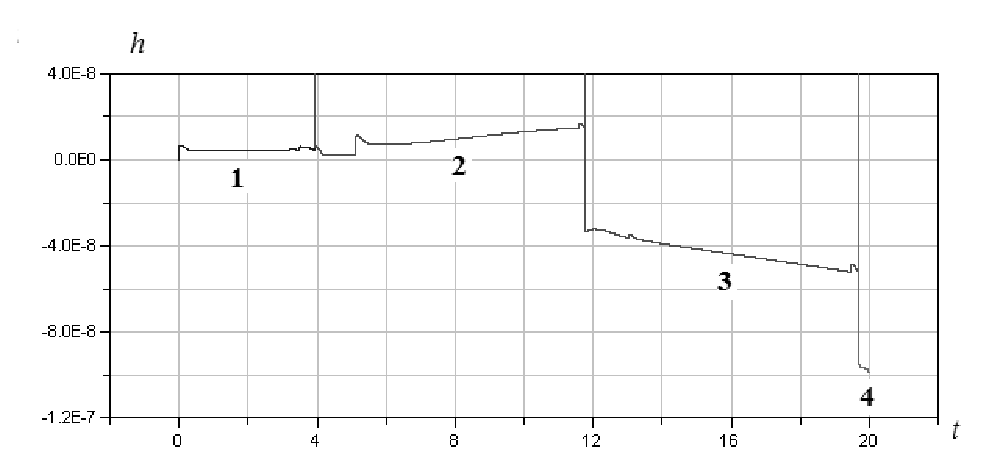
\includegraphics[width=15cm]{content/parts/3_friction/nd/Figure21.eps}}
\caption{Точность сохранения неудерживающей связи.}
\label{fig2}
\end{figure}

\subsection{Качественное сравнение модели с вязким трением и безынерционной модели}

Для модели с вязким трением были проведены расчеты, аналогичные движению 3 из главы 2. Конфигурация экипажа также симметрична, ролики усечены, на каждом колесе пять роликов.

Обнаружены динамические эффекты, аналогичные показанным в главе 2: характерный спиральный вид траектории центра масс на опорной плоскости возникает и в данной модели; видно раскручивание роликов; возрастание угловой скорости платформы экипажа, одновременное с убыванием поступательной скорости её центра; последующее медленное убывание угловой скорости; убывание кинетической энергии экипажа.

В данном расчете коэффициент вязкого трения принимался достаточно большим: $10^{5}$. Такое значение позволило моделировать ударный характер переходных процессов при смене ролика в контакте. На гладких участках движения сходство с движением неголономной модели соответствует результату \cite{karapetyan1981negolonom}.

\begin{figure}[htb]
\centerline{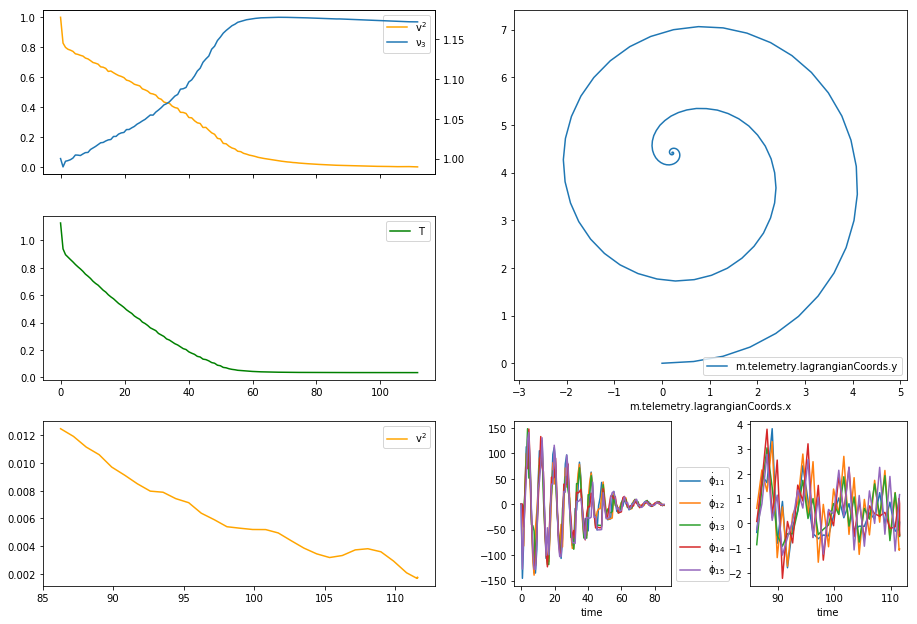
\includegraphics[width=\linewidth]{content/pic/new/visc_3_100.png}}
\caption{Характер движения системы с вязким трением при комбинации начальных условий движений 1 и 2. По оси абсцисс всюду, кроме правого верхнего графика отложено время}
\label{fig2}
\end{figure}
